%!LW recipe=XeLaTeXmk
\newif\ifbjut
\bjuttrue
\documentclass[scheme=plain,aspectratio=169]{ctexbeamer}
\usepackage[T1]{fontenc}
\usepackage{fontawesome5}
\usepackage{mathtools}
\usepackage{tikz}
\usepackage{booktabs}
\usepackage{caption}
\usepackage{outlines}
\usepackage{graphicx}
\usepackage{float}
\usepackage{amsthm}
\usepackage{tabularray}
\usepackage{minted}
\usepackage{hyperref}
\usepackage{cleveref}
\usepackage{url}
\usepackage{xspace}
\usepackage{academicons}
\usepackage{pgfplots}
\usepackage{pgfgantt}
\usepackage{qrcode}
\usepackage{ninecolors}
\usepackage{xltxtra}
\usepackage{tcolorbox}
\usepackage{tikz}
\tcbuselibrary{minted}
\tcbset{listing engine=minted}

\usetikzlibrary{fit}
\usetikzlibrary{calc}
\usetikzlibrary{arrows}
\usetikzlibrary{positioning}

\tikzstyle{arrow} = [-latex',->, to path={-- (\tikztotarget)}]
\tikzstyle{darrow} = [-latex',->, to path={-- (\tikztotarget)},double]
\usetheme[
    progressbar=frametitle,
    numbering=fraction,
    subsectionpage=progressbar,
    titleformat title=smallcaps,
    titleformat subtitle=smallcaps,
    titleformat section=smallcaps,
    titleformat frame=smallcaps]{metropolis}


\ifbjut
\definecolor{bjutblue}{HTML}{429ABF}
\definecolor{bjutbluelight}{HTML}{C5EAF3}
\definecolor{bjutbluedark}{HTML}{0096C3}
\setbeamercolor{palette primary}{bg=bjutblue}
\setbeamercolor{frametitle}{bg=bjutbluedark,fg=white}
\setbeamercolor{progress bar}{fg=bjutbluedark}
\else
\setbeamercolor{palette primary}{bg=gray1}
\setbeamercolor{frametitle}{bg=black,fg=white}
\setbeamercolor{progress bar}{fg=black}
\fi

\usetikzlibrary{calc}
\setcounter{tocdepth}{1}

\makeatletter
\newlength{\frametitle@padding}
\setlength{\frametitle@padding}{2.2ex}
\newcommand{\frametitlestrut@start}{
  \rule{0pt}{\frametitle@padding +%
    \totalheightof{%
      \ifcsdef{frametitleformat}{\frametitleformat X}{X}%
    }%
  }%
}

\newcommand{\frametitlestrut@end}{
  \rule[-\frametitle@padding]{0pt}{\frametitle@padding}
}

\setbeamertemplate{frametitle}{
    \nointerlineskip%
    \begin{beamercolorbox}[%
        wd=\paperwidth,%
        sep=0pt,%
        leftskip=\frametitle@padding,%
        rightskip=\frametitle@padding,%
      ]{frametitle}%
    \frametitlestrut@start%
    \insertframetitle%
    \hfill%
    \nolinebreak%
    \frametitlestrut@end%
    \end{beamercolorbox}%
    \begin{tikzpicture}[remember picture,overlay]
        \coordinate (logo) at ([xshift=-1.8cm,yshift=-0.6cm]current page.north east);
        \node at (logo) {\includegraphics[height=.1\textheight]{%
          \ifbjut bjutwhite.pdf\else northeastern.eps\fi%
        }};
    \end{tikzpicture}
}
\makeatother


\setbeamertemplate{footline}{
    \hbox{%
    \begin{beamercolorbox}[wd=\paperwidth,ht=3ex,dp=1.5ex,leftskip=2ex,rightskip=2ex]{page footer}%
        \usebeamerfont{title in head/foot}%
        \hfill
        \begin{tblr}{
            width=.8\linewidth,
            colspec={X[l]X[c]X[r]}
        }
            \insertsectionhead{}
            &
            \ifx\insertsubsection\empty
            \else
            \insertsubsection{} 
            \fi
            &
            \insertframenumber{} / \inserttotalframenumber
        \end{tblr}
        \hfill{}
    \end{beamercolorbox}}%
}

\defbeamertemplate{section page}{my progressbar}{
  \centering
  \begin{minipage}{22em}
    \raggedright
    \usebeamercolor[fg]{section title}
    \usebeamerfont{section title}
    \insertsection\\[-1ex]
    \usebeamertemplate*{progress bar in section page}
    \par
    \ifx\insertsubsectionhead\@empty\else%
      \usebeamercolor[fg]{subsection title}%
      \usebeamerfont{subsection title}%
      \insertsubsectionhead
    \fi
  \end{minipage}
  \par
  \vspace{\baselineskip}
}
\setbeamertemplate{section page}[my progressbar]
\let\OriginLaTeX\LaTeX
\renewcommand\LaTeX{\textrm{\OriginLaTeX\xspace}}

\UseTblrLibrary{booktabs}
\graphicspath{ {./images/} }

\title{LaTeX and Academic Typesetting}
\author{Yuxuan Lu}
% \institute{Northeastern Human-Centered AI Lab}
\ifbjut
\institute{北京工业大学程序设计集训队}
\else
\institute{Northeastern Human-Centered AI Lab}
\fi

\date{Feb. 5 2024}

\begin{document}

\maketitle

\begin{frame}{Takeaways \& Timeline}
    \begin{outline}
        \1 15-minute tutorial
        \1 30-minute interactive exercise
    \end{outline}
\end{frame}

\ifbjut
\begin{frame}{Who am I}
    \begin{outline}
        \Large
        \1 卢雨轩
        \normalsize
        \1 \url{https://yuxuan.lu}
        \1 北工大2019级; 计算机科学与技术实验班; 荣誉学士学位
        \1 美国东北大学 Ph.D. Student in Computer Science
        \1 前北工大程序设计集训队队长(2019-2023)
        \1 ICPC 铜牌 \texttimes 3; IEEE Xtreme World Rk 41, 85 (top 2\% and 3.5 \%)
        \1 负责2项国创、1项星火
        \1 本科期间在国际学术会议或期刊发表论文5篇
    \end{outline}
\end{frame}
\fi

\begin{frame}{Overall Introduction}
    \begin{outline}
        \1 What is \LaTeX?
            \2 Some ``Fancy'' and ``Anti-human'' text editor?
            \2 Some language describing math formula?
            \2 Some paper writing system that only researchers use?
    \end{outline}
\end{frame}
\begin{frame}{What is \LaTeX}
    \begin{outline}
        \1 What is Word
            \2 Microsoft Word is a word processor developed by Microsoft.
            \2 What-you-see-is-what-you-get, ``wysiwyg''
            \1 How about \LaTeX?
            \2 LaTeX is a high-quality typesetting system
        \pause
        \1 What's a typesetting system?
            \tiny
            \2 Typesetting is the composition of text for publication, display, or distribution
            \normalsize
            \ifbjut
            \2 活字印刷术
            \fi
            \2 Adobe InDesign
    \end{outline}
\end{frame}

\begin{frame}{Compare \LaTeX with Word}
    \begin{figure}
        \centering
        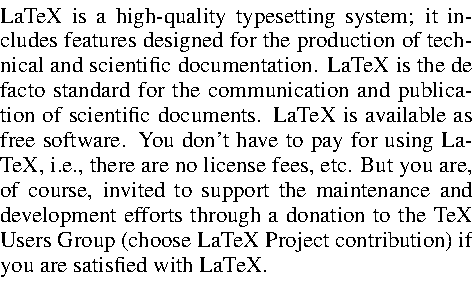
\includegraphics[width=.4\linewidth]{knuth-line-breaking-demo.pdf} %
        \hspace{1cm}
        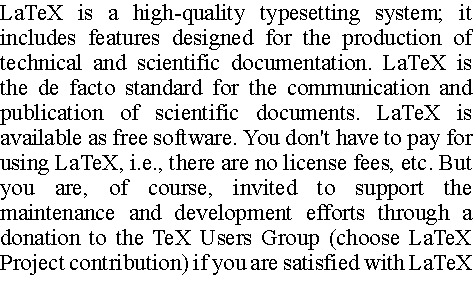
\includegraphics[width=.4\linewidth]{knuth-line-breaking-demo-word.pdf}
        \caption{Comparing \LaTeX with Word}
    \end{figure}
\end{frame}

\begin{frame}{History of \LaTeX}
    \begin{outline}
        \1 \textrm{\TeX} was developed by Donald Knuth for typesetting his book ``The art of computer programming''
        \ifbjut (计算机程序设计艺术) \fi
            \2 At that time, math formulas was mostly written and typesetting by hand
        \1 Leslie Lamport created \LaTeX
            \2 A set of macro defined around \textrm{\TeX}
            \2 Provide high-level concepts, like ``document class'' and ``packages''
        \1 \textrm{\XeLaTeX, \LuaLaTeX}, ...
    \end{outline}
\end{frame}

\begin{frame}{How to pronounce \LaTeX}
    \begin{outline}
        \1 TeX's official pronounciation is `tech'
            \2 X is $\chi$ as in $\chi^2$ distribution
        \1 Lay - TeX?
        \1 Lah - TeX?
        \1 LaTeX?
        \1 Personally I think it doesn't matter
            \2 ``The correct way to pronounce SQL is how your professor pronounces it''
    \end{outline}
\end{frame}

\begin{frame}{What \LaTeX features}
    \begin{outline}
        \1 Out-of-the-box experience
        \1 Easy-to-use ``seperation of content and presentation''
            \2 You can easily switch to another template within 30 minutes
        \1 Integrate with other softwares
            \2 Code highlighting
            \2 And even code execution
    \end{outline}
\end{frame}

\begin{frame}[fragile]{Examples}
    \begin{tcblisting}{}
\begin{minted}{python}
import os
import something_else
print("easy-to-use syntax highlighting!")
\end{minted}
    \end{tcblisting}
\end{frame}

\begin{frame}[fragile]{Examples}
    \begin{figure}
        \resizebox{!}{5cm}{\begin{tikzpicture}
            \node (0) {};
            \node (lexer) [below=.5cm of 0]{ Lexical Analyzer};
            \node (parser) [below=.5cm of lexer] { Syntax Analyzer};
            \node (semantic) [below=.5cm of parser] { Semantic Analyzer};
            \node (intermediate) [below = .5cm of semantic] { Intermediate Code Generate};
            \node (optimise) [below= .5cm of intermediate] { Optimiser};
            \node (1) [below=.5cm of optimise] { Object Code Generator};
            \node (2) [below=.5cm of 1] {};
            \draw [darrow] (0) -- node[right]{} (lexer);
            \draw [darrow] (lexer) -> node[right]{} (parser);
            \draw [darrow] (parser) -> node[right]{} (semantic) ;
            \draw [darrow] (semantic) -> node[right]{(AST)} (intermediate) ;
            \draw [darrow] (intermediate) -> node[right]{} (optimise) ;
            \draw [darrow] (optimise) -> node[right]{} (1) ;
            \draw [darrow] (1) -> node[right]{} (2) ;   
        
            
            \node [draw=black, thick, densely dotted,inner ysep=0,fit=(0) (lexer) (parser) (semantic) (intermediate) (optimise),label=left:{frontend},color=purple!70!white] {};
        
            \node [draw=red!30!black, thick, densely dotted,inner ysep=0,fit=(optimise) (1) (2),label=left:{backend}] {};
        \end{tikzpicture}}
    \end{figure}
\end{frame}

\begin{frame}
    \begin{figure}[htp]
      \centering
      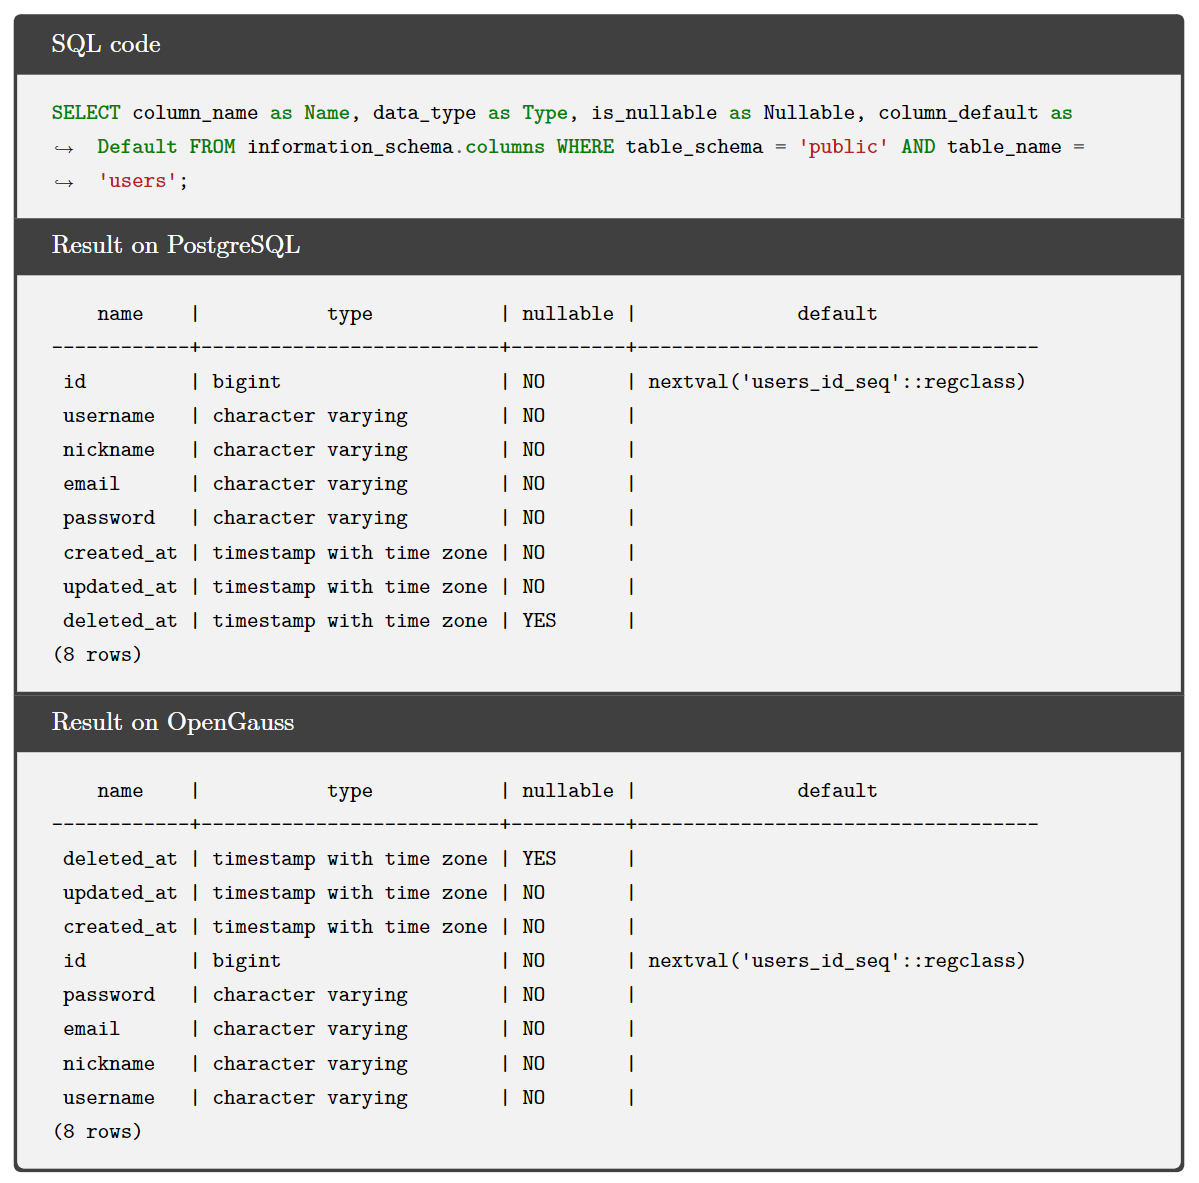
\includegraphics[width=.5\linewidth]{image1.png}
      \caption{And -- Even run and render results from other software}
    \end{figure}
\end{frame}

\begin{frame}[standout]
    This slide itself!
\end{frame}

\begin{frame}{Is \LaTeX good?}
    \begin{outline}
        \1 Nope!
            \2 Macro-based syntex isn't friendly
            \2 It'll took a day to find a missing brace (\})
        \1 New challengers:
            \2 Typst
    \end{outline}
\end{frame}

\begin{frame}{When to use \LaTeX}
    \begin{outline}
        \1 When to use \LaTeX
            \2 Academic publishing
            \2 Fine-grain typesetting
                \3 Course Project Report
            \2 Just for fun
        \1 When not to use \LaTeX
            \2 Homeworks
                \3 Use Markdown with LaTeX theme
            \2 Drawing diagrams
            \2 Whenver you don't feel like
    \end{outline}
\end{frame}

\begin{frame}[standout]
    Questions?
\end{frame}

\end{document}


